\section{Design and Implementation}

We tried to build multi-label classifier with DNN and light gradient boosting machine (LGBM). This section describes how each model is built and how it works.

\subsection{DNN}

We implemented multi-label DNN classifier by using  tensorflow API \cite{tensorflow_api}. Though tensorflow provides predefined DNN classifier, we need to build a custom DNN classifier to train the dataset and evaluate the model. Since predefined DNN classifier is capable to use the input feature which has same structure. However, there can be different number of mutations for a cancer which cannot be used for predefined DNN classifier. There is a choice that preprocess input dataset which row is a tensor indicating multiple mutations for a sample, which column length is same with the number of human genes. The preprocessed dataset, however, takes too much volume of storage to maintain the dataset. We want to make a model which is scalable, but the dataset may cause out of memory to load whole dataset or low performance to load partial input data.

\begin{figure}[t]
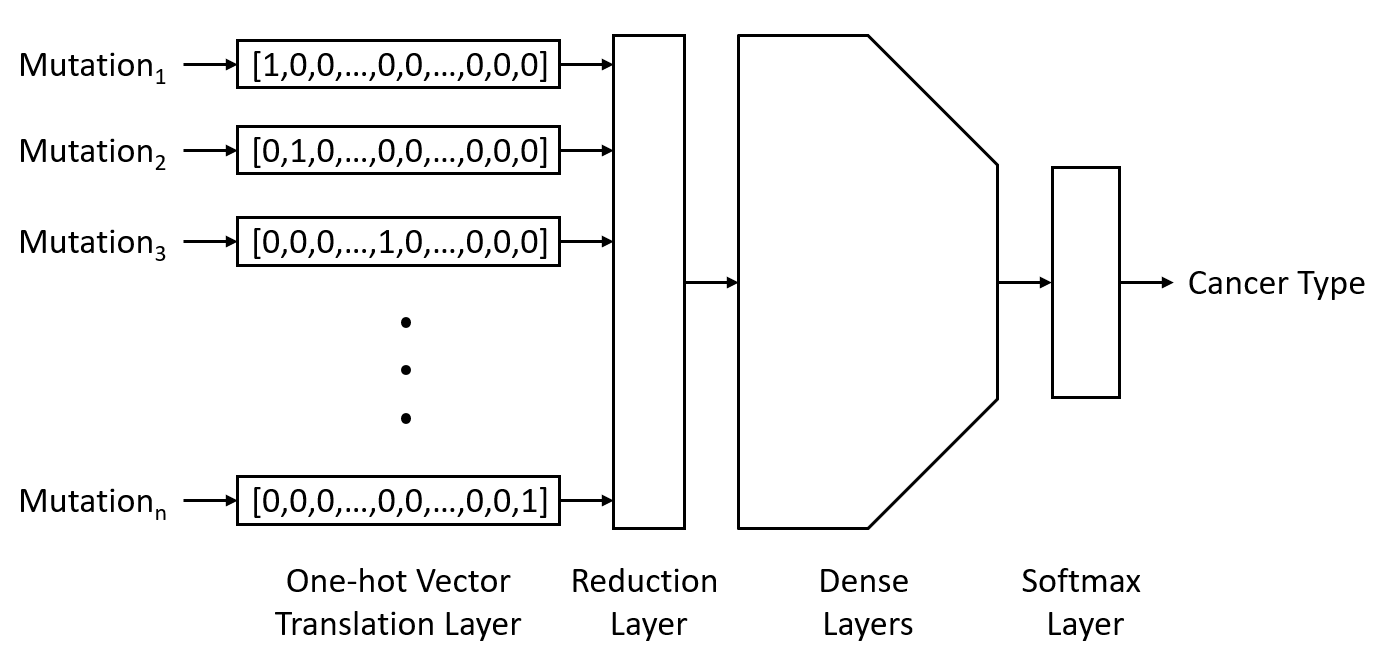
\includegraphics[width=0.48\textwidth]{figs/overview_dnn_model.png}
\caption{Custom DNN model overview}
\label{fig:overview_dnn_model}
\end{figure}

Our custom DNN classifier consumes arbitrary number of mutations for a sample and predict the cancer type of the sample. Figure~\ref{fig:overview_dnn_model} shows the overview of the model. The input of the model is a batch which includes all mutations for a sample. Each mutation is translated to an one-hot vector in the ont-hot vector translation layer. The model reduces one-hot vectors to a single vector in the reduction layer indicating whether the gene had been mutated or not; 0 for normal gene, 1 for mutated gene. The reduced tensor becomes a input tensor for dense layers. We use fully connected neural network for 13 dense layers with 0.5 dropout. We use linear function for activation, because sigmoid and rectified linear unit (ReLU) functions  converge too fast which causes overfitting problem.

The result of dense layers are converted to a tensor with 6 variables by using softmax function in the softmax layer. the softmax function calculates the portion of each tensor element and it is widely-used multi-label classifier. We selected the most highest possibility of cancer type with the output to calculate the accuracy of the model. We use sigmoid cross entropy to calculate loss which is an error between expected value with estimated value and we use ADADELTA \cite{zeiler2012adadelta} to optimize the model which changes the weights of dense layers in the direction of reducing the loss of the model.

\subsection{LightGBM}

We also implement a multiclass classifier by using LightGBM~\cite{ke2017lightgbm,meng2016communication}. LightGBM is a fast and high-performance gradient boosting framework based on decision tree algorithms, which is mainly used for machine-learning tasks including classification and ranking. It has been developed as a part of the Distrubuted Machine Learning Toolkit (DMLT) project~\cite{dmtk_project} of Microsoft and recently showed outstanding achievments~\cite{lightgbm_examples} in various machine learning challenges.


\begin{figure}[t]
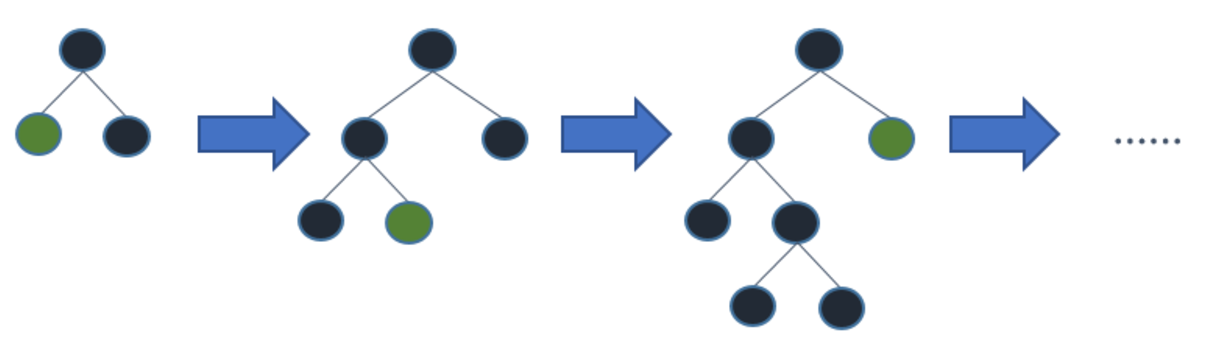
\includegraphics[width=0.48\textwidth]{figs/leaf-wise_tree_growth.png}
\caption{Leaf-wise tree growth of LightGBM~\cite{lightgbm_guide}}
\label{fig:leaf-wise_tree_growth}
\end{figure}

\begin{figure}[t]
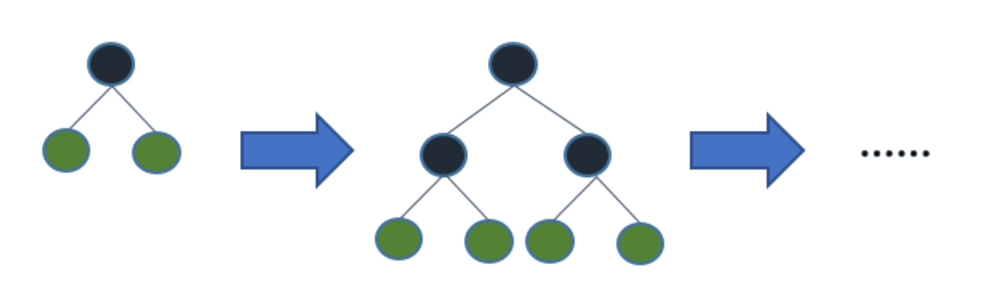
\includegraphics[width=0.48\textwidth]{figs/level-wise_tree_growth.png}
\caption{Level-wise tree growth of other boosting algorithms~\cite{lightgbm_guide}}
\label{fig:level-wise_tree_growth}
\end{figure}

One of the important design characteristics of LightGBM is the use of the leaf-wise tree grows. Figure~\ref{fig:leaf-wise_tree_growth} and Figure~\ref{fig:level-wise_tree_growth} shows the tree growth of LightGBM and other boosting algorithms. While other algorithms grow tree horizontally (i.e., level-wise), LightGBM grows tree vertically (i.e., leaf-wise). As a result, LightGBM can achieve lower loss than other level-wise boosting algorithms for the same number of leaves.

Another important characteristic of LightGBM is Exclusive Feature Bundling (EFB). EFB is effective for reducing the number of features. In many real-world applications with a large number of features, the feature space are often sparse. The cancer type mutation list data used in this project also has a sparse feature space because we use one-hot encoding for the gene list to represent mutated genes (that is the reason why DeepGene~\cite{yuan2016deepgene} introduces the clustered gene filtering and indexed sparsity reducing techniques to improve the accuracy and speed of the classifier). LightGBM has an algorithm for merging exclusive features that can automatically reduces the number of features in the sparse feature space. 

\begin{table}
\caption{LightGBM parameters}
\centering
\begin{tabular}{|l||l|}
\hline
{\bf Parameter} & {\bf Value}\\
\hline
\hline
{\bf boosting\_type} & gbdt \\
\hline
{\bf objective} & multiclass \\
\hline
{\bf num\_class} & 6 \\
\hline
{\bf metric} & multi\_logloss \\
\hline
{\bf num\_leaves} & 255 \\
\hline
{\bf min\_data\_in\_leaf} & 200 \\
\hline
{\bf max\_depth} & 8 \\
\hline
{\bf max\_bin} & 255 \\
\hline
{\bf num\_leaves} & 255 \\
\hline
{\bf subsample\_for\_bin} & 1000000 \\
\hline
{\bf learning\_rate} & 0.01 \\
\hline
{\bf num\_boost\_round} & 5000 \\
\hline
\end{tabular}
\label{tab:lightgbm_parameters}
\end{table}

LightGBM provides many tuning parameters for the leaf-wise tree growth algorithm, including \textit{num\_leaves} (i.e., maximum number of leaves in one tree), \textit{min\_data\_in\_leaf} (i.e., minimal number of data in one leaf), and \textit{max\_depth} (i.e., limitation of the maximum depth for tree model). While LightGBM can converge much faster than other level-wise tree growth algorithms, the tuning parameters should be carefully determined to avoid over-fitting. Table~\ref{tab:lightgbm_parameters} summarizes the baseline settings for the LightGBM parameters used in this project. We set the parameters on the basis of the parameter tuning guide, a multiclass classification example code provided by the official LightGBM code repository, and machine learning challenge winning solutions based on LightGBM.

Two important considerations of the parameter tuning are the trade-off between the training speed and the model accuracy and the over-fitting. We focus on the model accuracy rather than the training speed because LightGBM provides reasonable performance with the used dataset even when the performance-centric settings are used.
